
\begin{center}
	\Huge
	Kurvelængde
\end{center}
\section*{Kurvelængde for vektorfunktioner}
\stepcounter{section}

Vi så i integralregning at kurvelængden for en differentiabel funktion $f$ på et interval $[a,b]$ er givet ved
\begin{align*}
	\int_a^b \sqrt{1+f'(x)}dx.
\end{align*}
Vi vil betragte det mere generelle tilfælde: kurvelængden for en vektorfunktion $\vv{r}:\mathbb{R}\to \mathbb{R}^2$. 

\begin{setn}[Kurvelængde]
	Lad $\vv{r}:\mathbb{R} \to \mathbb{R}^2$ være en vektorfunktion givet ved
	\begin{align*}
		\vv{r}(t) = 
		\begin{pmatrix}
			x(t)\\
			y(t)
		\end{pmatrix},
	\end{align*}
	hvor $x$ og $y$ begge er differentiable samt at $x'$ og $y'$ er kontinuerte. Så er kurvelængden $L$ for parameterkurven på $t$-intervallet $[a,b]$ givet ved integralet
	\begin{align*}
		L = \int_a^b\sqrt{x'(t)^2+y'(t)^2}dt.
	\end{align*}
\end{setn}
\begin{proof}
	Vi lader $L_a(t)$ betegne kurvelængden af parameterkurven for $\vv{r}$ på $t$-intervallet $[a,b]$. Lad desuden $h>0$ være givet. Vi approksimerer længden af linjestykket $L_t(t+h)$ med længden af 
	den rette linje mellem punkterne.
	\begin{align*}
		L_t(t+h) \approx \sqrt{(x(t+h)-x(t))^2+(y(t+h)-y(t))^2}.		
	\end{align*}
	Der må altså gælde for $t>a$, at 
	\begin{align*}
						&L_ a(t+h) = L_a(t) + \sqrt{(x(t+h)-x(t))^2 + (y(t+h)-y(t))^2} + \varepsilon \\
		\Leftrightarrow \ & L_a(t+h) -L_a(t) = \sqrt{(x(t+h)-x(t))^2 + (y(t+h)-y(t))^2} + \varepsilon  \\
		\Leftrightarrow \ & \frac{L_a(t+h) -L_a(t)}{h} = \frac{\sqrt{(x(t+h)-x(t))^2 + (y(t+h)-y(t))^2}}{h} +  \frac{\varepsilon}{h} \\
		\Leftrightarrow \ & \frac{L_a(t+h) -L_a(t)}{h} = \sqrt{\frac{(x(t+h)-x(t))^2}{h^2} + \frac{(y(t+h)-y(t))^2}{h^2}} + \frac{\varepsilon}{h}  \\
		\Leftrightarrow	\ & \frac{L_a(t+h) -L_a(t)}{h} = \sqrt{\left(\frac{x(t+h)-x(t)}{h}\right)^2 + \left(\frac{(y(t+h)-y(t))}{h}\right)^2}  + \frac{\varepsilon}{h}
	\end{align*}
	Størrelsen $\varepsilon$ er den fejl, vi får ved vores lineære approksimation af linjestykket. 
	Vi tager nu grænseværdien $\lim_{h\to 0}$ på begge sider af lighedstegnet. Vi får, at
	\begin{align*}
		\lim_{h\to 0} \frac{x(t+h)-x(t)}{h} = x'(t),
	\end{align*}
	og
	\begin{align*}
		\lim_{h \to 0} \frac{y(t+h)-y(t)}{h} = y'(t),
	\end{align*}
	da $x$ og $y$ er antaget differentiable. Derfor får vi i alt, at $L_a(t)$ er differentiabel og, at
	\begin{align*}
		\lim_{h\to 0} \frac{L_a(t+h)-L_a(t)}{h} = L_a'(t) = \sqrt{x'(t)^2 +y'(t)^2},
	\end{align*}
	da det kan vises, at når $x'(t)$ og $y'(t)$ begge er kontinuerte, så går $\varepsilon/h$ mod $0$ for $h$ gående mod $0$. 
	Dermed er $L_a(t)$ en stamfunktion til $\sqrt{x'(t)^2+y'(t)^2}$ og vi har for følgende bestemte integral, at 
	\begin{align*}
		\int_a^b \sqrt{x'(t)^2+y'(t)^2} dt = L_a(b)-L_a(a) = L_a(b),	
	\end{align*}
	hvilket var hvad vi skulle vise, da $L_a(b)$ netop betegner længden af kurven når $t$ løber fra $a$ til $b$.
\end{proof}
Da der i kurvelængdeformlen indgår en kvadratrod under integraltegnet, er integralerne oftest meget svære at løse, og har tit ikke nogle løsninger, der kan repræsenteres ved gængse funktioner. Vi vil derfor næsten altid approksimere kurvelængder ved brug af et CAS-værktøj som Maple.

\begin{exa}
	Vi ønsker at bestemme kurvelængden af vektorfunktionen $\vv{r}: \mathbb{R} \to \mathbb{R}^2$ givet ved
	\begin{align*}
		\vv{r}(t) = 
		\begin{pmatrix}
			t^2-1 \\
			t^4+4t
		\end{pmatrix}.
	\end{align*}
	Et plot af parameterkurven for $\vv{r}$ hvor $t\in [-2,2]$ kan ses af Fig. \ref{fig:kurvelaengde}.
	\begin{figure}[H]
		\centering
		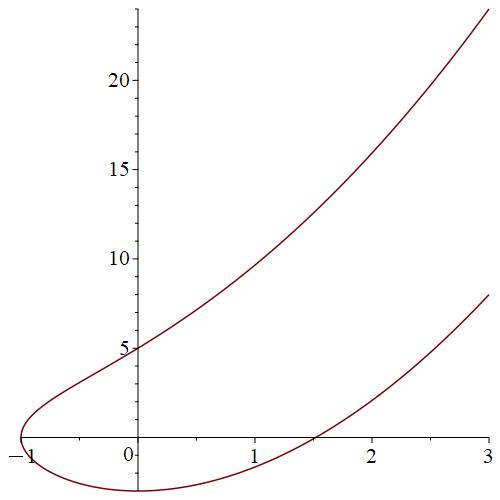
\includegraphics[width=0.7\textwidth]{Billeder/kurvelaengde.jpg}
		\caption{Parameterkurve}
		\label{fig:kurvelaengde}	
	\end{figure}
	Vi ønsker at bestemme kurvelængden for parameterkurven for $\vv{r}$ på intervallet $[-2,2]$. Vi skal derfor løse integralet
	\begin{align*}
		L &= \int_{-2}^2 \sqrt{x'(t)^2+y'(t)^2}dt \\
		&=\int_{-2}^2\sqrt{(2t)^2+(4t^3+4)^2} dt.
	\end{align*}
	Dette løses i Maple og vi får
	\begin{align*}
		L \approx 39.32.
	\end{align*}
	(Bemærk, at det er vigtigt at skrive -2.0 og 2.0 i integralgrænserne, da Maple ellers vil forsøge at løse integralet eksakt.)
\end{exa}

\section*{Opgave 1}
I de følgende opgaver prøv gerne at tegne vektorfunktionerne før I bestemmer kurvelængderne. 
\begin{enumerate}[label=\roman*)]
	\item En vektorfunktion $\vv{r}$ er givet ved
	\begin{align*}
		\vv{r}(t) = 
		\begin{pmatrix}
			\ln(t) \\
			e^t
		\end{pmatrix}.
	\end{align*}
	Bestem kurvelængden af parameterkurven for $\vv{r}$ på $t$-intervallet $[0,5]$.
	\item En vektorfunktion $\vv{r}$ er givet ved
	\begin{align*}
		\vv{r}(t) = 
		\begin{pmatrix}
			\cos(t) \\
			\sin(t)
		\end{pmatrix}.
	\end{align*}
	Bestem kurvelængden af parameterkurven for $\vv{r}$ på $t$-intervallet $[\pi,\pi]$. 
	\item En vektorfunktion $\vv{r}$ er givet ved
	\begin{align*}
		\vv{r}(t) = 
		\begin{pmatrix}
			t^2+t \\
			t^3-10t^2
		\end{pmatrix}.
	\end{align*}
	Bestem kurvelængden af parameterkurven for $\vv{r}$ på $t$-intervallet $[-1,2]$. 
	\item En vektorfunktion $\vv{r}$ er givet ved
	\begin{align*}
		\vv{r}(t) = 
		\begin{pmatrix}
			t^2+3 \\
			t^3-4t
		\end{pmatrix}.
	\end{align*}
	Bestem kurvelængden af parameterkurven for $\vv{r}$ på $t$-intervallet $[-2,2]$. 
\end{enumerate}

\section*{Opgave 2}
I 2.g lærte vi, at kurvelængden for en differentiabel funktion $f$ på intervallet $[a,b]$ er givet ved
\begin{align*}
	L = \int_a^b \sqrt{1+f'(x)}dx.
\end{align*}
Brug sætningen om kurvelængder for vektorfunktioner til at bevise dette. (Vink: opskriv $f(x)$ som en vektorfunktion. )
